\documentclass[11pt]{article}

\usepackage{mi_lab_include_2015-06-01}

\usepackage{times}
\usepackage{mathptm}
\usepackage{fullpage}
\usepackage{hyperref}
\usepackage{graphicx}

\begin{document}

\begin{center}
\medskip
{\bf{Computational Activity 4: Space, the Final Frontier}} 
\medskip

{\em{Derived from activites VP04 and VP05 in the instructor resources that
 accompany \\ Ruth Chabay and Bruce Sherwood's {\em Matter and Interactions} 
 textbook.}}
\medskip
\end{center}

In this activity, you will simulate motion with gravitational forces,
eventually building up a program that simulates the elliptical orbit of
a spacecraft.
You have previously written down a formula for the gravitational 
potential energy, $V_g = G m M / r$.  You have also seen that the 
gravitational force is opposite to the derivative of potential energy.
Extending that idea to three dimensions, we obtain that the gravitational
force is
\begin{displaymath}
{\vec F}_g = - G \frac{m M}{r^2} {\hat r}
\end{displaymath}
This formula is known as ``Newton's Law of Universal Gravitation.''  
The vector $\vec r$ is the displacement from the object creating the 
gravitational force to the object experiencing the gravitational force,
with $r = | \vec r | $ and $\hat r = \vec r / r$, 
Note that the vector $\hat r$ is a {\em unit vector} that points in the
radially outward direction, directly away from the other body.  
By definition, any unit vector has a magntitude of 1 (with no units!), so it
contains information only about the direction of the force, not about
its magnitude. (VPython hint: In VPython, if you have some vector \texttt{some\_vector}, then you can find its magnitude with \texttt{mag(some\_vector)}.)

\section{Prediction}

\begin{compactitem}[\color{MIRed}$\Rightarrow$]
\item On a whiteboard draw a diagram like the one below.  Each numbered dot represents the position of a different spacecraft. (A single spacecraft near a planet would not move in a straight line.)
\item At each numbered location draw an arrow representing the gravitational force on a spacecraft at that location, due to the planet.
\item Make sure that your diagram makes sense.  Is the direction of each arrow correct? Is the length of the arrow proportional to the magnitude of the quantity it represents?\\
\end{compactitem}

\begin{center}
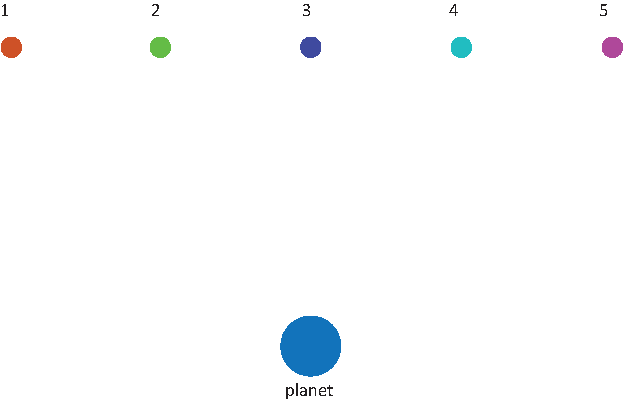
\includegraphics{planet_5_spacecraft.pdf}
\end{center}

\vspace*{10pt}
%\checkpoint

\section{Objects and Constants}

\subsection{Creating Objects}

\begin{compactitem}[\color{MIRed}$\Rightarrow$]
\item Start a VPython program by inserting these lines at the beginning:\\
\color{CodeColor}
\begin{verbatim}
scene.width = 1000
\end{verbatim}
\color{black}
\vspace*{10pt}
\item Create a sphere of radius \po{6.4}{6} m, located at \mivec{0,\po{-2}{7},0} m to represent the planet. Give the sphere an appropriate name.
\item Create a second sphere to represent the spacecraft. Give this sphere an appropriate name. You will need to exaggerate its radius to make it visible; try \po{3}{6}~m.  Place it at location \mivec{\po{-13}{7},\po{4.5}{7},0}~m, and make its color different from the color of the planet.
\end{compactitem}

\subsection{Constants}

In a program it is important to use symbolic names for constants.  Why?  To make it easy to make changes and corrections to the model.  For example, if you want to change the mass of an object, it is much easier to change a single line such as :

\color{CodeColor}
\begin{verbatim}
mass = 1.3e7
\end{verbatim}
\color{black}

than it is to search for and replace all occurrences of the string \color{CodeColor}\texttt{1.3e7}\color{black}.\\

\begin{compactitem}[\color{MIRed}$\Rightarrow$]
\item Insert a line of code that assigns the name ``G'' to the value of the gravitational constant.
\item Also create approriately named variables to store the masses of the planet (\po{6}{24} kg) and of a spacecraft (\po{1.5}{4} kg).\\
\end{compactitem}

\section{Calculating Gravitational Force}

For the single spacecraft your program has created:\\
\begin{compactitem}[\color{MIRed}$\Rightarrow$]
\item Add instructions to calculate gravitational force on the spacecraft by the planet. Use symbolic names for every quantity in the program lines you write.
\item Print the value you calculated.  Does the direction of the force make sense?
\end{compactitem}

\subsection{Representing Gravitational Force with an Arrow}  

\begin{compactitem}[\color{MIRed}$\Rightarrow$]
\item Create an \code{arrow} object with its tail at the location of the spacecraft.  
\item Set the \code{axis} of the \code{arrow} object to the value of the gravitational force you calculated.
\item Run the program.  What do you see?  Can you explain why?
\end{compactitem}

\subsection{Scale Factors}

We will frequently want to use \code{arrow} objects to visualize vector quantities such as forces.  However, if the distances between objects in the program is very large compared to the magnitude of the vector, the \code{arrow} may be too small to see.  (Alternatively, if the distance between objects is very small compared to the magnitude of the vector, the \code{arrow} object may be so huge that no other objects can be seen.)\\

\begin{compactitem}[\color{MIRed}$\Rightarrow$]
\item Watch the VPython instructional video \textit{VPython Instructional Videos: 5. Scale Factors }\\ \url{http://vpython.org/video05.html} to see how to multiply the \code{axis} attribute of an \code{arrow} by a scalar to adjust its length so all objects in the scene are visible.
\item Use an appropriate scale factor to scale your \code{arrow} to an appropriate length.  Be prepared to explain how you determined this scale factor.\\
\end{compactitem}

%\checkpoint

\section{Multiple Locations}

To calculate and display the gravitational force on several spacecraft at different locations, as in the diagram you drew previously, we can use a loop.  Recall that in a previous activity you encountered loops that moved a single object. We could also create loops  that create multiple objects at different locations. \\ 

\begin{compactitem}[\color{MIRed}$\Rightarrow$]
\item Which of the following loops, Loop 1 or Loop 2, will create multiple different objects? 
\item Which loop will move a single object across the screen?\\
\end{compactitem}

 
Loop 1

\color{CodeColor}
\begin{Verbatim}[frame=single]  
wall = box(pos=vector(0,0,-2), length=40, height=20, width=1)
x = -20
dx = 2
ball = sphere(pos = vector(x,0,0), color=color.red, radius=0.3)
while x < 21:
    rate(2)
    ball.pos = ball.pos + vector(dx,0,0)
    x = x + dx
\end{Verbatim}
\color{black}

Loop 2:

\color{CodeColor}
\begin{Verbatim}[frame=single]
wall = box(pos=vector(0,0,-2), length=40, height=20, width=1)
x = -20
dx = 2
while x < 21:
    rate(2)
    ball = sphere(pos = vector(x,0,0), color=color.red, radius=0.3)
    x = x + dx
\end{Verbatim}
\color{black}


\subsection{Gravitational Force at Multiple Locations}

Modify your program so that it contains a single \while loop which does the following:\\

\begin{compactitem}[\color{MIRed}$\Rightarrow$]
\item Creates five different spheres representing five spacecraft at these locations:\\
\mivec{\po{-13}{7}, \po{4.5}{7},0} m\\
\mivec{\po{-6.5}{7}, \po{4.5}{7},0} m\\
\mivec{0, \po{4.5}{7},0} m\\
\mivec{\po{6.5}{7}, \po{4.5}{7},0} m\\
\mivec{\po{13}{7}, \po{4.5}{7},0} m\\
\item Calculates and prints the gravitational force on each spacecraft by the planet.
\item Visualizes the gravitational force on each spacecraft with an \code{arrow} with its tail on the spacecraft. 
Adjust the scale factor to make the display comprehensible, but make sure you use the same scale factor for all arrows! 
To make it easier to compare arrows, set the \code{shaftwidth} of each \code{arrow} equal to half the radius of a planet.\\
\end{compactitem}

%\checkpoint


\section{Forces on the Planet}


 

\begin{compactitem}[\color{MIRed}$\Rightarrow$]
\item Modify your program so that it also displays 5 arrows representing the forces on the planet by the five spacecraft.
\item Make sure the directions and magnitudes of these arrows make sense.
%\item Turn in your program.\\
\end{compactitem}
% % % % % % % % % % % % % % % % % % % % % % % % % % % % %

\vspace{24pt}
\hrule

\newpage

\section{Explain and Predict}

Study the following VPython program carefully. Make sure you understand the whole program, but don't run the program yet. Reading and explaining program code is an important part of learning to create and modify computational models.

\color{CodeColor}
\begin{Verbatim}[frame=single]
scene.width = 800
scene.height = 800

G = 6.7e-11
mEarth = 6e24
mcraft = 15e3
deltat = 60

Earth = sphere(pos=vector(0,0,0), radius=6.4e6, color=color.cyan)
craft = sphere(pos=vector(-10*Earth.radius, 0,0), radius=1e6,
               color=color.yellow, make_trail=True)
vcraft = vector(0,2e3,0)
pcraft = mcraft*vcraft
t = 0
scene.autoscale = False ##turn off automatic camera zoom

while t < 10*365*24*60*60:
    rate(100)     
    craft.pos = craft.pos + (pcraft/mcraft)*deltat
    t = t+deltat
\end{Verbatim}
\color{black}

Without running the program, answer the following questions:

\begin{compactitem}[\color{MIRed}$\Rightarrow$]
\item What is the physical system being modeled? 
\item In the real world, how should this system behave? On the left side of your whiteboard or paper, draw a sketch showing how you think the objects should move in the real world. 
\item Will the program as it is now written accurately model the real system?
\item On the right side of the whiteboard or paper, draw a sketch of how the objects created in the program will move on the screen, based on your interpretation of the code.
\end{compactitem}


%\checkpoint

\section{Modify and Extend the Model}

\begin{compactitem}[\color{MIRed}$\Rightarrow$]
\item Run the program.   
\item How did your prediction compare to what you saw? Did something happen that you didn't expect to happen?
\item How should the program be changed so that it is a physically reasonable model of the system?
\item Modify the program.  Run it and compare its behavior to the behavior you expect from the real system.
\end{compactitem}

%\checkpoint

\section{Visualize Momentum}

In a previous activity, you used arrows to visualize gravitational force vectors. In this program, you will use an arrow to visualize the momentum of the spacecraft.  Note that you want one arrow that moves with the spacecraft--you don't want to create many arrows.  Therefore you will create the arrow before the loop, and change its \code{pos} and \code{axis} inside the loop, just after updating the \code{pos} of the spacecraft.  You may review the video on scale factors if necessary: \textit{VPython Instructional Videos: 5. Scale Factors } \url{http://vpython.org/video05.html}\\

\begin{compactitem}[\color{MIRed}$\Rightarrow$]
\item Print the initial momentum of the spacecraft. 
\item Use this value to decide on a value for a scale factor that will make the arrow representing momentum a reasonable length in the display.
\item Before the computational loop:
\begin{compactitem}[\color{MIRed}$\Rightarrow$]
\item Add a line of code that assigns the symbolic name \code{sf} to the scale factor.   
\item Create an arrow named \code{parr} to represent the craft's momentum.
\end{compactitem}
\item Inside the loop, add two lines of code (after the position update) like this:\\\\
\hspace{20pt}\code{parr.pos = craft.pos}\\
\hspace{20pt}\code{parr.axis = pcraft * sf}\\

\item Once you have seen the entire orbit, you may have to adjust the scale factor.
\end{compactitem}

\section{Testing a Value of a Variable}

An \code{if} statement can be used to instruct VPython to do something only in a particular situation.  The action to take is indented after the \code{if} statement.  For example, consider the following code fragment:

\color{CodeColor}
\begin{Verbatim}[frame=single]
a = 3
if a < 4:
    sphere(color=color.green)
box(pos=vector(3,3,0), color=color.cyan)
\end{Verbatim}
\color{black}

\begin{compactitem}[\color{MIRed}$\Rightarrow$]
\item Try the code above in a new program window.  What does it do?   
\item What happens when you replace \code{a = 3} with \code{a = 8}?
\end{compactitem}

\subsection{Detecting a Collision}

If your spacecraft collides with the Earth, the program should stop.\\

\begin{compactitem}[\color{MIRed}$\Rightarrow$]
\item Add code similar to the following inside your loop (using the name you defined for the relative position vector between the spacecraft and the center of the Earth):   
\end{compactitem}


\color{CodeColor}
\begin{Verbatim}
if mag(r) < Earth.radius:
     break  ## exit from the loop
\end{Verbatim}
\color{black}

The \code{break} instruction tells VPython to get out of the loop and go to the first instruction after the loop (if there is one.)  Because the \code{break} instruction is indented after the \code{if} statement, it will be executed only if the \code{if} test returns a value of \code{True}.


\section{Direction of Momentum}

Record your answers to the following questions:\\

\begin{compactitem}[\color{MIRed}$\Rightarrow$]
\item For this elliptical orbit, what is the direction of the spacecraft's momentum vector? Tangential? Radial? Something else?
\item What happens to the momentum as the spacecraft moves away from the Earth?   
\item As it moves toward the Earth?
\item Why? Explain these changes in momentum in terms of the Momentum Principle.
\end{compactitem}


\section{Effect of the Initial Velocity}

\begin{compactitem}[\color{MIRed}$\Rightarrow$]
\item Approximately, what minimum initial speed is required so that the spacecraft ``escapes'' and never comes back? You may have to zoom out to see whether the spacecraft shows signs of coming back. You may also have to extend the time in the while statement.
\item What initial speed is required to make a nearly circular orbit around the Earth? You may wish to zoom out to examine the orbit more closely.   
\item How does increasing the initial speed affect the orbit? Explain this by considering the first few time steps.
\item How does decreasing the initial speed affect the orbit? Explain this by considering the first few time steps.
\end{compactitem}

\section{Adding an Arrow to Represent Force }

\begin{compactitem}[\color{MIRed}$\Rightarrow$]
\item Choose an initial speed that produces an elliptical orbit.
\item Add a second, different colored arrow representing the net force on the spacecraft.  This arrow should also move with the craft.  You'll need a different scale factor for this arrow.
\item Are the net force on the craft and the momentum of the craft in the same direction?
\item What is the relative direction of these arrows when the craft is slowing down?  
\item Speeding up?  
\item Draw a diagram showing the directions of the craft's momentum and the net force on the craft at 6 different locations along an elliptical orbit. At each location note whether the speed of the craft is increasing, decreasing, or momentarily not changing.
\end{compactitem}


%\section{Turn in Your Program}
%
%Choose an initial speed that produces an elliptical orbit.  Turn in your program and the answers to the questions posed above.
\vspace{24pt}
\hrule


\end{document}
